\documentclass[tikz]{standalone}
\usepackage{amsmath}

\begin{document}

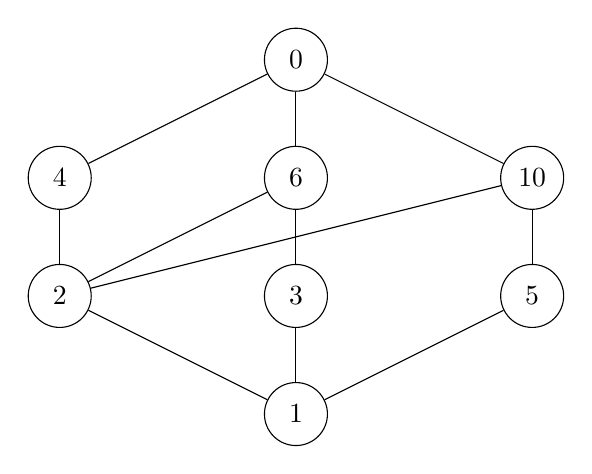
\begin{tikzpicture}[node distance=1.5cm, every node/.style={draw, circle, minimum size=0.8cm, inner sep=0pt}]
    % Nodes
    \node (1) at (0,0) {1};
    \node (2) at (-3,1.5) {2};
    \node (3) at (0,1.5) {3};
    \node (5) at (3,1.5) {5};
    \node (4) at (-3,3) {4};
    \node (6) at (0,3) {6};
    \node (10) at (3,3) {10};
    \node (0) at (0,4.5) {0};
    
    % Edges
    \draw (1) -- (2);
    \draw (1) -- (3);
    \draw (1) -- (5);
    \draw (2) -- (4);
    \draw (2) -- (6);
    \draw (2) -- (10);
    \draw (3) -- (6);
    \draw (5) -- (10);
    \draw (4) -- (0);
    \draw (6) -- (0);
    \draw (10) -- (0);
\end{tikzpicture}

\end{document}